% Chapter Template

\chapter{User studies} % Main chapter title

\label{Chapter6} % Change X to a consecutive number; for referencing this chapter elsewhere, use \ref{ChapterX}

\lhead{Chapter 6. \emph{User experience evaluation}} 
Human-Robot Interaction (HRI) being a rapidly advancing area of research, there is a growing need for strong experimental designs and methods of evaluation. This will bring credibility and validity to scientific research that involves humans as subjects, as recognized in the psychology and social science fields. As robots are becoming more prevalent, accurate methods to assess how humans respond to robots, how they feel about their interactions with robots, and how they interpret the actions of robots are very important. 

\section{Experiment}

\subsection{Protocol}
\begin{figure}[H]
\centering
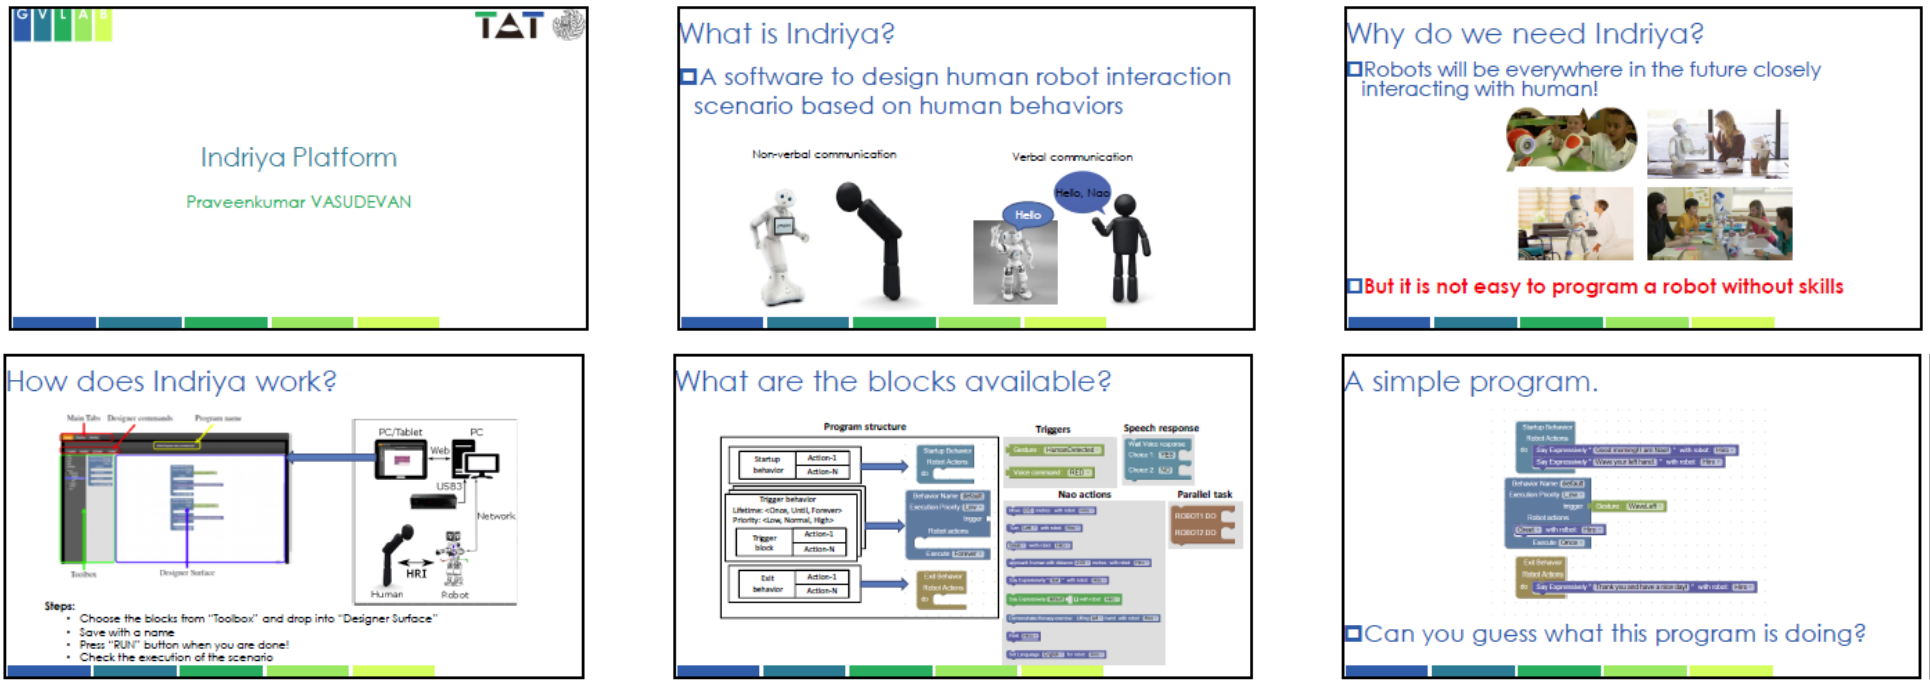
\includegraphics[width=0.8\textwidth]{../thesis/assets/handout.png}
\caption[System description handout]{System description handout}
\label{fig:handout}
\end{figure}
\section{Summary and Discussion}